\documentclass[a4paper, 10pt, twocolumn]{article}
\usepackage{amssymb}
\usepackage{cellspace, graphicx, makecell}
\usepackage{graphicx} % Required for inserting images
\usepackage[utf8]{inputenc}
\usepackage[T2A]{fontenc}
\usepackage[english,russian]{babel}
\usepackage{cmap}
\usepackage[left=1cm,right=1cm,
    top=1cm,bottom=2cm]{geometry}
\usepackage{paracol}
\usepackage{multicol}
\usepackage{amsmath}
\usepackage{lipsum}
\usepackage{vwcol}
\usepackage{float}

% Установка размера формул
\DeclareMathSizes{10}{10}{10}{10}   % Для основного текста размером 10pt

\title{Лабораторная работа 2.1.6 \\ Измерение удельной теплоёмкости воздуха при постоянном
давленини}
\author{Матвей Галицын \\ Б01-411}
\date{March 15, 2025}

\setlength{\columnseprule}{0.1pt}
\setlength{\columnsep}{3em}
\raggedbottom
\begin{document}
\maketitle
\newpage{}
\section{Аннотация}

    \subsection{Задача}
    В работе измеряются изменения температуры углекислого газа при протекании
    через малопроницаемую перегородку при разных начальных значениях. По полученным данным 
    вычисляются коэфиициенты газа Ван-дер-Ваальса 

    \subsection{Оборудование}
    Трубка с пористой перегородкой; труба Дьюара; термостат, термометры; дифференицальная 
    термопара; микровольтметр; балластный баллон; манометр.

\section{Теория}
    Рассмотрим стационарный поток газа между произвольными сечениями трубки
    и пористой перегородкой. Для 1 моля можно записать первое начало термодинамики:

    $$ A_1 - A_2 = \left(U_2 + \frac{\mu v_2^2}{2}\right) - \left(U_1 + \frac{\mu v_1^2}{2}\right) \eqno{(1)}$$

    где $A_1 = P_1V_1$ -- работа над газом, необходимая для внесения его в 
    первое сечение трубки, $A_2 = P_2V_2$ -- работа газа по прохождению второго
    сечения. Используя уравнение (1), получим: 

    $$ H_1 - H_2 = (U_1 + P_1V_1) - (U_2 + P_2V_2) = \frac{1}{2}\mu (v_2^2 - v_1^2) \eqno{(2)}$$

    Или:

    $$ C_P(T_1 - T_2) = \frac{1}{2}\mu (v_2^2 - v_1^2) $$

    откуда:

    $$ \Delta T = \frac{\mu}{2C_P}(v_2^2 - v_1^2)\eqno{(3)} $$

    При этом:

    $$ v_1 = \frac{P_2}{P_1}v_2 \eqno{(4)} $$

    Таким образом, для углекислого газа оценка по формуле (3) дает 
    $\Delta T = 7 \cdot 10^{-4}$ К, что ничтожно мало по сравнению с измеряемым
    эффектом. 

    \paragraph{Эффект Джоуля-Томсона} Для дифференциального эффекта Джоуля-Томсона
    имеем:

    $$ \Delta T = \frac{\frac{2a}{RT} - b}{C_P}\Delta P \eqno(5)$$
    
    где $a$ и $b$ -- коэффициенты в уравнении Ван-дер-Ваальса:

    $$ \left(P + \frac{a}{V^2}\right)(V - b) = RT \eqno{(6)} $$
    
    Таким образом, $a$ и $b$ можно получить из нескольких пар значений 
    $(\mu, T)$, где
    $$ \mu = \frac{\frac{2a}{RT} - b}{C_P} \eqno{(7)} $$

    Через коэффициенты Ван-дер-Ваальса находим температуру инверсии эффекта
    Джоуля-Томсона:
    $$ T_i = \frac{2a}{Rb} \eqno{(8)} $$

    Критическая точка газа определяется условиями:
    $$ \left(\frac{\partial P}{\partial V}\right)_T = 0, \ \left(\frac{\partial^2 P}{\partial V^2}
    \right)_T = 0 $$,
    откуда, используя уравнение (6), получим все параметры газа в
    критической точке:
    $$ V_{\text{к}} = 3b, \ T_{\text{к}} = \frac{8a}{27Rb}, \ P_{\text{к}} = \frac{a}{27b^2} $$

    Связывая формулы (6) и (7), получим:
    $$ T_i = \frac{27}{4}T_{\text{к}} $$
    
\section{Экспериментальная установка}
    Экспериментальная установка. Схема установки для исследования эффекта Джоуля Томсона в углекислом 
    газе представлена на рисунке. Основным элементом установки является трубка 1 с пористой 
    перегородкой 2, через которую пропускается исследуемый газ. Трубка имеет длину 80 мм и сделана из нержавеющей стали, обладающей, как известно, малой теплопроводностью. Диаметр трубки 4 = 3 мм, толщина стенок 0,2 мм. Пористая перегородка расположена в конце трубки и
    представляет собой стеклянную пористую пробку со множеством узких и длинныых каналов.
    \begin{figure}[H]
        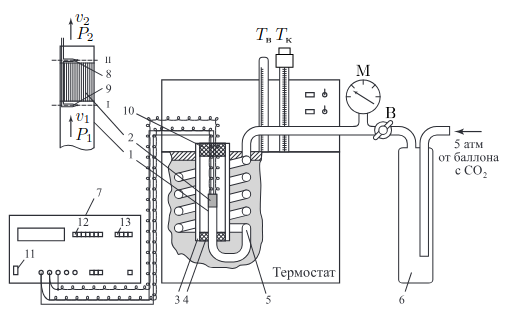
\includegraphics[width=1\linewidth]{images/installation.png}
        \begin{center}
            \caption{Экспериментальная установка}
        \end{center}
    \end{figure}
    Пористость и толщина пробки (1 = 5 мм) подобраны так, чтобы обеспечить оптимальный поток газа 
    при перепаде давлений $\Delta P < 4$ атм (расход газа составляет около 10 $\text{см}^3/\text{с}
    $); при этом в
    результате эффекта Джоуля-Томсона создаётся достаточная разность температур. Углекислый газ под 
    повышенным давлением поступает в трубку через змеевик 5 из балластного баллона 6. Медный 
    змеевик омывается водой и нагревает медленно протекающий через него газ до температуры 
    воды в термостате. Температура воды измеряется термометром $T_\text{в}$, помещённым в 
    термостате. Требуемая температура воды устанавливается и поддерживается при помощи контактного 
    термометра $T_k$. Давление газа в трубке измеряется манометром М и регулируется вентилем В (при 
    открывании вентиля В, т. е. при повороте ручки против часовой стрелки, давление Р повьпнается). 
    Манометр М измеряет разность между давлением внутри трубки и наружным (атмосферным).
    Так как углекислый газ после пористой перегородки переходит в область с атмосферным давлением 
    $ P_2 $, то этот манометр непосредственно измеряет перепад давления на входе и на выходе трубки
    $\Delta P = P_1 - P_2$ 

    Разность температур газа до перегородки и после неё измеряется дифференциальной термопарой медь 
    — константан. Константановая проволока диаметром 0,1 мм соединяет спаи 8 и 9, а медные 
    проволоки (того же диаметра) подсоединены к пифровому вольтметру 7. Отвод тепла через проволоку 
    столь малого сечения пренебрежимо мал. Для уменьшения теплоотвода трубка с пористой 
    перегородкой помещена в трубу Дьюара 3, стенки которой посеребрены, для уменьшения теплоотдачи, 
    связанной с излучением. Для уменьшения теплоотдачи за счёт конвекции один конец трубы Дьюара 
    уплотнен кольцом 4, а другой за крыт пробкой 10 из пенопласта. Такая пробка практически не 
    создает перепада давлений между внутренней полостью трубы и атмосферой.

\section{Результаты измерений и обработка данных}
    Далее приведены результаты экспериментов при T = 27 °C, 47 °C, 67 °C.
    Сразу за каждой таблицей идет график зависимости $\Delta T(\Delta p)$. \newline
    Угловой коэффициент касательной можно расчитывать по методу наименьших квадратов.
    $$k = \frac{\left\langle \Delta T \cdot \Delta p \right\rangle}
    {\left\langle {\Delta p}^2 \right\rangle}$$
    % Смещение по вертикали: $$R_0 = \left\langle R \right\rangle - k \cdot \left\langle Q \right\rangle^2$$
    Таблица №1 $\Delta T \text{~от~} \Delta P$ приведена в приложении. \newline
    График: 
    Коэффициенты наклона:
        $$ k_1 = \frac{7.78}{11.74} = 0.66 \text{ К/атм} $$
        $$ k_2 = 0.5 \text{ К/атм} $$
        $$ k_3 = 0.46 \text{ К/атм} $$

    \begin{figure}[H]
        \centering
        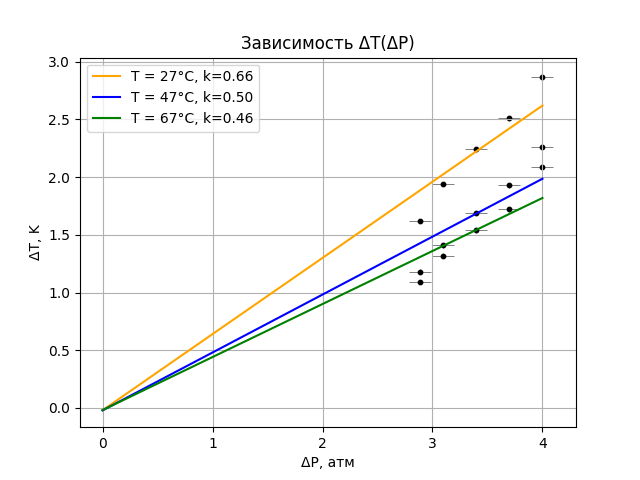
\includegraphics[width=1\linewidth]{graphs/figure1.png}
        \begin{center}
            \caption{График зависимости при $\Delta T \text{~от~} \Delta P$}
        \end{center}
    \end{figure}
    Таким образом, получаем таблицу №2, приведенную в приложении. \newline
    Соответствующий график:

    \begin{figure}[H]
        \centering
        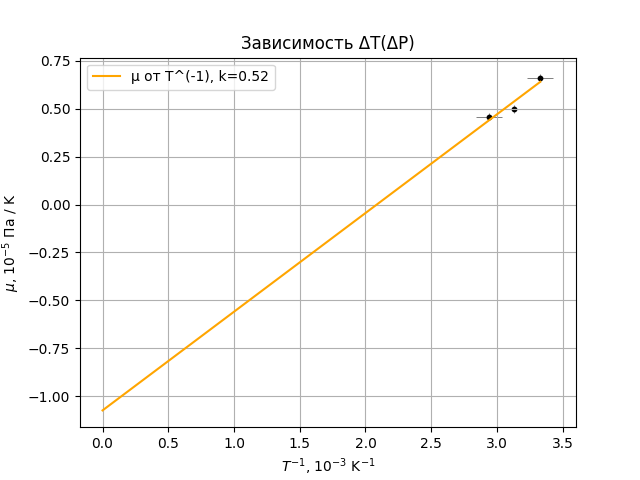
\includegraphics[width=1\linewidth]{graphs/figure2.png}
        \begin{center}
            \caption{Зависимость $\mu$ от $T^{-1}$ }
        \end{center}
    \end{figure}
    Коэффициент наклона в данном случае: $$ k = 0.52 \cdot 10^{-2} \text{ Па}$$
    $$\sigma_k = \frac{1}{\sqrt{n}} \cdot \sqrt{\frac{\left\langle \mu^2 \right\rangle - \left\langle \mu \right\rangle^2}
    {\left\langle \left({T^{-1}}\right)^2 \right\rangle - \left\langle \left({T^{-1}}\right) \right\rangle^2} - k }$$
    $$\sigma_k = \frac{1}{\sqrt{3}}\cdot \sqrt{\frac{0.3*10^{-10}}{9.91*10^{-6}} - 0.52*10^{-2}} \approx 0.05 \cdot 10^{-2} \text{ Па}$$
    Смещение по вертикали: $$ b = -1.07 \cdot 10^{-5}$$

    Так как данный графиик отображает следующую зависимость $ \mu = \frac{2a}{RC_P} \cdot T ^{-1} - \frac{b}{C_P}$, то коэффициент наклона это $\frac{2a}{RC_P}$, а смещение это $-\frac{b}{C_P}$.

    Отсюда $$ a = 0.75 \pm 0.15 \frac{\text{Па} \cdot \text{м}^6}{\text{К} \cdot \text{моль}^2} $$
    $$b = (4.25 \pm 0.78) 10^{-4} \frac{\text{м}^3}{\text{моль}}$$
    По формуле (8) получаем температуру инверсии: $$ T_i = 424 \text{К}$$

\section{Обсуждение результатов}
    В результате работы мы:
    \begin{itemize}
        \item Выявили экспериментально наличие эффекта Джоуля-Томсона,
        показали его линейность с неплохой степенью точности.

        \item Вычислили коэффициенты $a$ и $b$, мы обнаружили расхождение с табличными значениями на целый порядок, поэтому наш опыт показывает, что модель газа Ван-дер-Ваальса способна описывать поведение газа лишь при малых отклонениях температуры.

        \item Получили значение температуры инверсии $T_i$
    \end{itemize}
    \newpage
\onecolumn
\section{Приложение}

\begin{table}[H]
    \centering
    \begin{tabular}{|c|c|c|c|c|c|} \hline
    № & $\Delta T$, K & $\Delta U, \text{мкВ} $ & $\Delta p, \text{атм}$ &
     $ \Delta T \cdot \Delta P, \text{К} \cdot \text{атм} $ & $ {\Delta P}^2, \text{атм}^2 $ \\ 
     \hline

    \multicolumn{6}{|c|}{\text{T = 27 °C}} \\ \hline
    1 & 2.87 & 117 & 4   & 11.48 & 16     \\ \hline
    2 & 2.51 & 102 & 3.7 & 9.29  & 13.69  \\ \hline
    3 & 2.24 & 91  & 3.4 & 7.62  & 11.56  \\ \hline
    4 & 1.94 & 79  & 3.1 & 6.01  & 9.61   \\ \hline
    5 & 1.62 & 66  & 2.8 & 4.54  & 7.84   \\ \hline
    \shortstack{Среднее \\ значение} & 2.23 & & 3.4 & 7.78 & 11.74 \\ \hline

    \multicolumn{6}{|c|}{\text{T = 47 °C}} \\ \hline
    1 & 2.26 & 96 & 4   & 9.04 & 16       \\ \hline
    2 & 1.93 & 82 & 3.7 & 7.14 & 13.69    \\ \hline
    3 & 1.69 & 72 & 3.4 & 5.75 & 11.56    \\ \hline
    4 & 1.41 & 60 & 3.1 & 4.37 & 9.61     \\ \hline
    5 & 1.18 & 50 & 2.8 & 3.30 & 7.84     \\ \hline
    \shortstack{Среднее \\ значение} & 1.55 & & 3.4 & 5.92 & 11.74 \\ \hline

    \multicolumn{6}{|c|}{\text{T = 67 °C}} \\ \hline
    1 & 2.09 & 92 & 4   & 8.36 & 16       \\ \hline
    2 & 1.72 & 76 & 3.7 & 6.36 & 13.69    \\ \hline
    3 & 1.54 & 68 & 3.4 & 5.24 & 11.56    \\ \hline
    4 & 1.32 & 58 & 3.1 & 4.09 & 9.61     \\ \hline
    5 & 1.09 & 48 & 2.8 & 3.05 & 7.84     \\ \hline
    \shortstack{Среднее \\ значение} & 1.55 & & 3.4 & 5.42 & 11.74 \\ \hline

    \end{tabular}
    \caption{Таблица зависимости $\Delta T(\Delta p)$ при T = 27 °C, 47 °C, 67 °C}
\end{table}

\begin{table}[H]
    \centering
    \begin{tabular}{|c|c|c|c|c|c|} \hline
    № & $T, ^\circ\text{C}$ & $T^{-1},~10^{-3}\frac{1}{\text{К}}$ & $\mu,~10^{-5}~\text{К / Па}$ & $\left(T^{-1}\right)^2,~10^{-6}\frac{1}{\text{К}^2}$ & $\mu^2,~10^{-10}~\left(\text{К / Па}\right)^2$ \\ \hline
    1 & 27 & 3.33 & 0.66 & 11.09 &  0.44\\ \hline
    2 & 47 & 3.13 & 0.50 & 9.79  &  0.25\\ \hline
    3 & 67 & 2.94 & 0.46 & 8.84  &  0.21\\ \hline
    \shortstack{Среднее \\ значение} & & 3.13 & 0.54 & 9.91 & 0.30\\ \hline

    \end{tabular}
    \caption{Зависимость $\mu(T^{-1})$ при T = 27 °C, 47 °C, 67 °C}
\end{table}

\end{document}